\ylDisplay{Lennukid} % Ülesande nimi
{Tundmatu autor} % Autor
{piirkonnavoor} % Voor
{2014} % Aasta
{P 9} % Ülesande nr.
{3} % Raskustase
{
% Teema: Mehaanika
\ifStatement
Kaks lennukit lendavad samal kõrgusel kiirustega $v_1 = 800$ $km/h$ ja $v_2 = 600$ $km/h$. Vaadeldaval hetkel on lennukite liikumise sihid omavahel risti ning kumbki lennuk paikeb sihtide ristumispunktist kaugusel $a = 20$ $km$. Leidke, milline on lennukite vähim vahekaugus järgneva liikumise jooksul, kui eeldada, et kumbki lennuk kurssi ei muuda.\fi


\ifHint
Lahendus muutub lihtsaks, kui vaatleme ühe lennuki suhtelist liikumist teise suhtes ehk kui kujutame mõtteliselt punase lennukiga $B$ kaasaliikuvat taustsüsteemi.
\fi

\ifSolution
Lahendus muutub lihtsaks, kui vaatleme ühe lennuki suhtelist liikumist teise suhtes. Nimelt, lähme mõtteliselt punase lennukiga $B$ kaasaliikuvasse taustsüsteemi. Sel juhul paistab lennuk $B$ paigal püsivat, kuid lennuk $A$ näib liikuvat kiirusega $\vec{v}$, mille komponendid on joonisel välja toodud. Kiiruse mooduli leiame Pythagorase teoreemist: $v = 1000$ km/h. Vähim kaugus kahe lennuki vahel kogu liikumise jooksul on mõistagi trajektoorini tõmmatud ristlõik $BX$, mille pikkuse järgnevalt leiamegi.
\begin{center}
	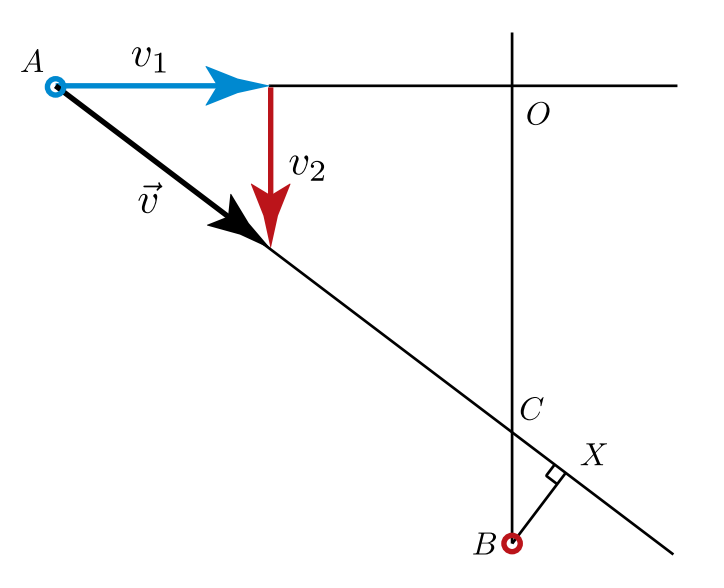
\includegraphics[width=0.5\linewidth]{2014-v2p-09-lah.png}
\end{center}
Punkti $C$ jõudes oli lennuk $A$ ida-lääne sihis liikunud vahemaa \textbar$AO$\textbar$ $ $= a = 20$ km ning põhja-lõuna sihis järelikult \textbar $OC$\textbar $ $ $= v_2 \cdot a/v_1 = 15$ km
Järelikult \textbar{$BC$}\textbar = $a$ - \textbar{$OC$}\textbar = $5$ km.
Kolmnurga $BCX$ ning kiirusvektorite kolmikust moodustatud kolmnurga küljepikkuste võrdelisusest leiame meid huvitava pikkuse.
\begin{center}
\textbar $BX$\textbar $= \frac {v_1\cdot\mid{BC}\mid}{v} = 4 km$
\end{center}
Võib arvutada ka pikkuse $\mid$AC$\mid$ ning kasutada kolmnurkade $BCX$ ja $ACO$ sarnasust.
\fi
}